\documentclass[crop,tikz]{standalone}
	\usetikzlibrary{patterns}
\begin{document}
	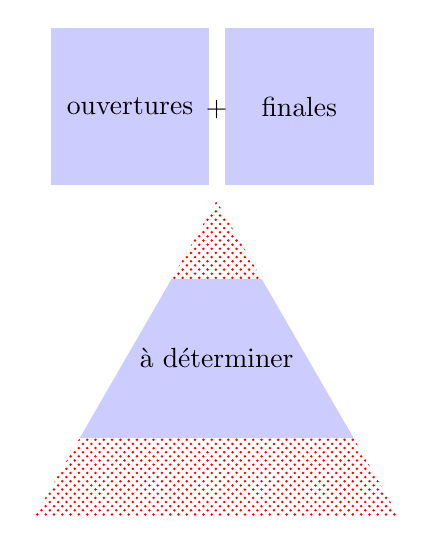
\begin{tikzpicture}
		\fill[color=blue!20] (-2.1, 3.2) rectangle (-0.1,5.2) node[color=black,pos=.5] {ouvertures};
		\fill[color=blue!20] (0.1, 3.2) rectangle (2,5.2) node[color=black,pos=.5] {finales};
		\draw (0,4.4) node[below]{$+$} ;
 		\begin{scope}
 		\clip (-1,2) rectangle (1,3);
 		\fill[pattern=crosshatch dots, pattern color=red] (90:3cm) \foreach \x in {210,330} {
 			-- (\x:3cm)
 		} -- cycle (60:3cm) ;
 		\end{scope}
		\begin{scope}
			\clip (-2,0) rectangle (2,2);
			\fill[color=blue!20] (90:3cm) \foreach \x in {210,330} {
				-- (\x:3cm)
			} -- cycle (0,1) node[color=black]{\`{a} d\'{e}terminer} ;
		\end{scope}
		
		\begin{scope}
			\clip (-2.4,-1) rectangle (2.4,0);
			\fill[pattern=crosshatch dots, pattern color=red] (90:3cm) \foreach \x in {210,330} {
				-- (\x:3cm)
			} -- cycle (60:3cm) ;
		\end{scope}
	\end{tikzpicture}
\end{document}